\section{Demonstration}\label{sec:demonstration}
%Our demonstration consist of using datasets from open data portals for some cities in France. \figref{expMappingParking} shows some of our experiments using these datasets. For each city, we performed two experiment. In \kword{NK}, no keywords are added by the user while in \kword{WK}, keywords are added. As we can see, even without keywords, there are fields that can be correctly mapped. Obviously, with keywords, initial mappings with better quality are generated. For all these datasets, we have their respective schema descriptions that we intend to use in our demonstration. 



%\begin{figure}
%	\centering
%	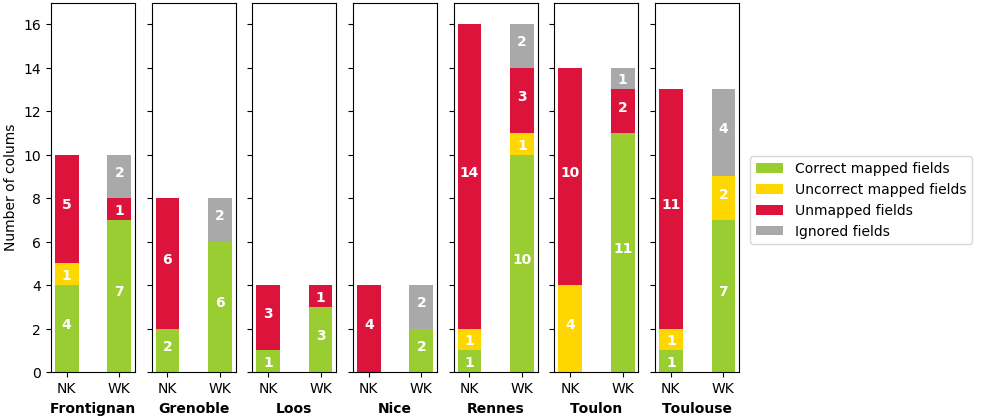
\includegraphics[scale=0.3]{./images/mappingPerParking1.png}
%	\caption{Mappings of the columns grouped per parking dataset. Where \emph{NK} represents the 
%		experiment without keywords and \emph{WK} represents the experiments with keywords.}
%	\label{fig:expMappingParking}
%\end{figure}

\begin{table}[]
    \centering
    \begin{tabular}{|c|c|c|c|c|c|c|c|c|c|c|}
        \hline
         & id & CODE & LIBELLE & ADRESSE & TYPE & TOTAL & type & id & lon & lat \\
        \hline
        NK & & & & & & & & & & \\
        \hline
        WK & & & & & & & & & & \\
        \hline
    \end{tabular}
    \caption{Caption}
    \label{tab:my_label}
\end{table}